\documentclass[UTF-8]{article}


\usepackage{booktabs}
\usepackage{url}
\usepackage{cite}
\usepackage[version=4]{mhchem}
\usepackage{graphicx}
\usepackage{subfigure}
\usepackage[a4paper,top=2cm,bottom=2cm,right=3cm,left=3cm,marginparwidth=1.75cm]{geometry}
\usepackage{amsmath}

\title{Protein Crystallization}
\author{Yan Haoming}
\date{October 25\\November 1\\2024}


\begin{document}
\maketitle

\section{Configuration of Influential Factors}
\begin{figure}
    \centering
    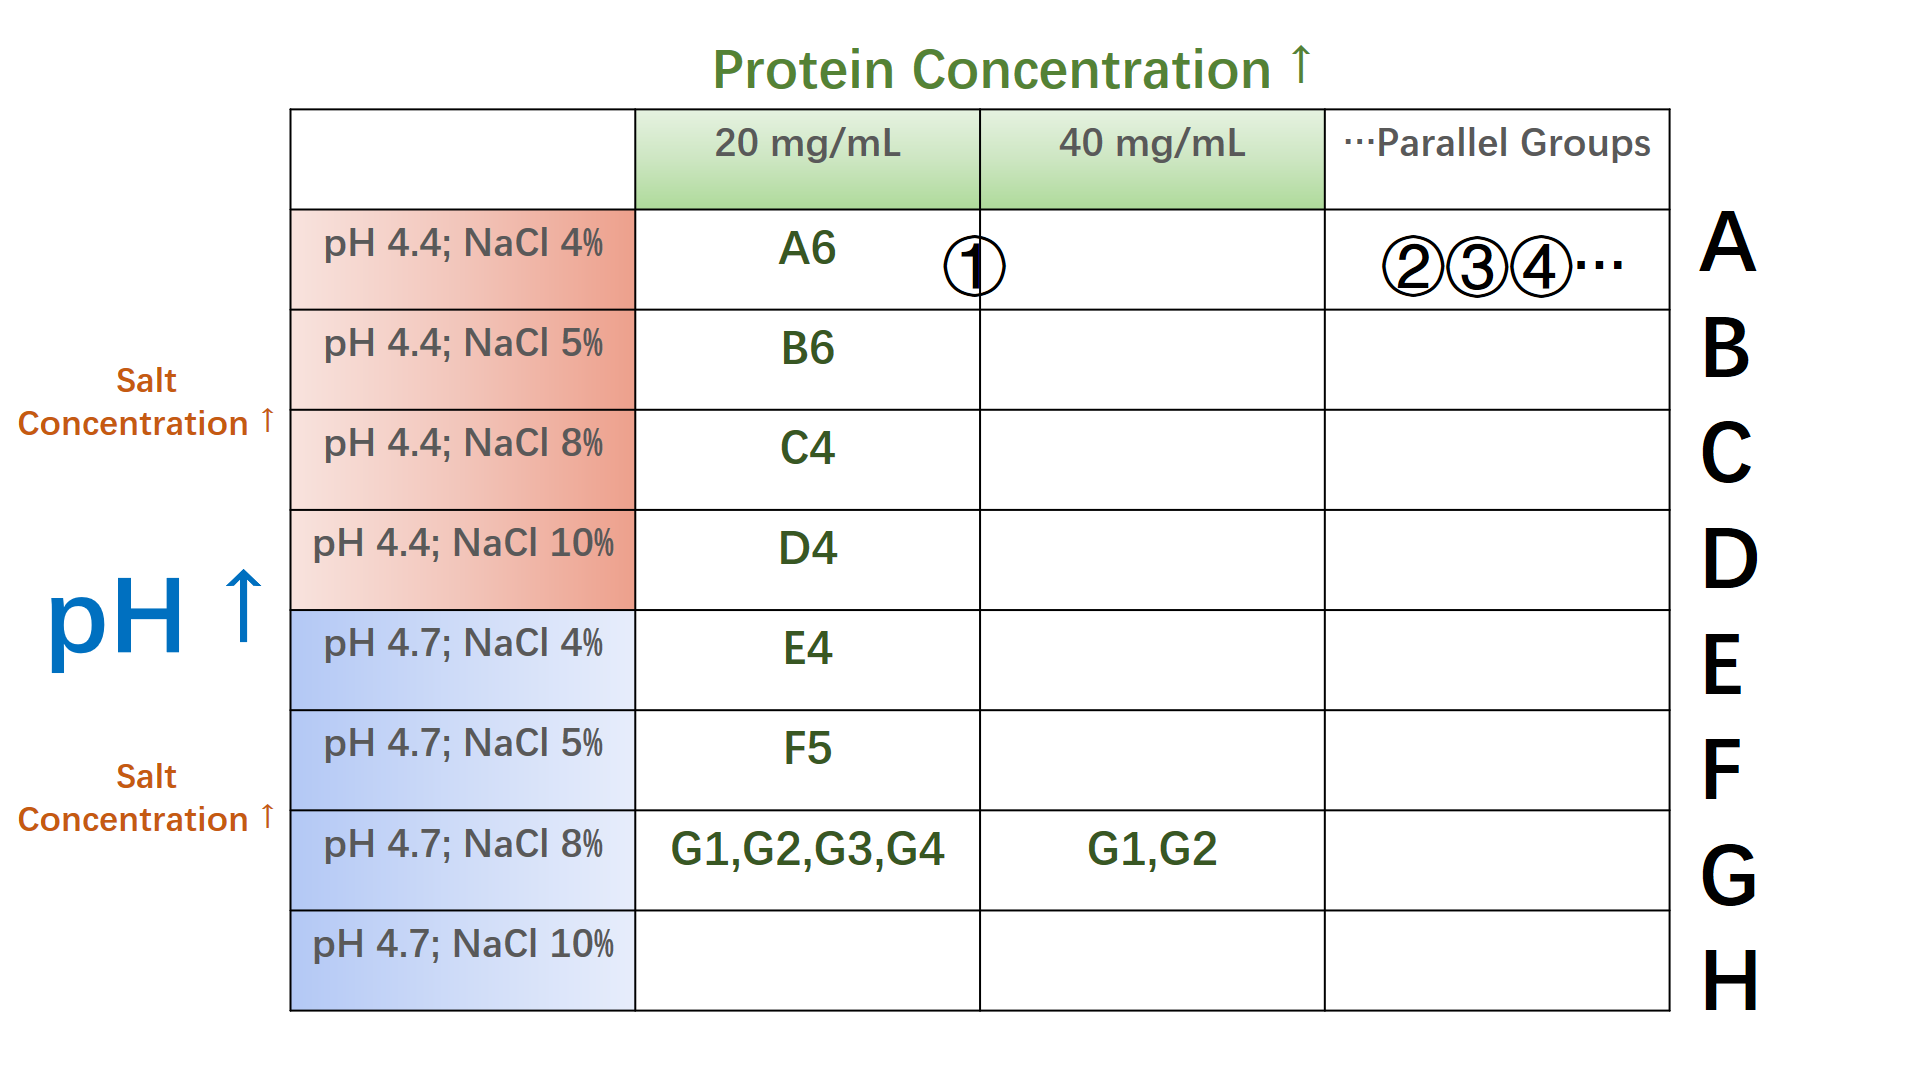
\includegraphics[width=1\linewidth]{../Figures/Configuration of Plate and Crystal Distribution.png}
    \caption{Configuration of Plate and Distribution of Crystals}
    \label{Configuration of Plate and Distribution of Crystals}
\end{figure}
\begin{figure}
    \centering
    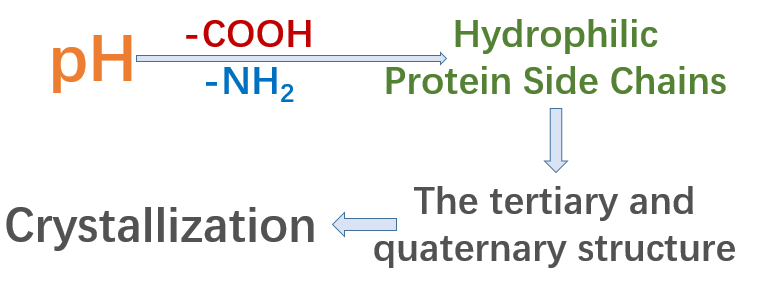
\includegraphics[width=1\linewidth]{../Figures/logic.png}
    \caption{The Influence of pH}
    \label{The Influence of pH}
\end{figure}
The process of developing protein crystals is influenced by many factors.
In this experiment, we changed pH, salt concentration(\ce{NaCl}) and protein concentration(lysozyme).

The configuration of those Influential factors can be seen in Figure \ref{Configuration of Plate and Distribution of Crystals}.
The cells in each row are in the same condition serving as the parallel groups.
The first four rows differ in salt concentration and same goes for the last four rows.
The pH is different between the first four rows and the last four rows as a whole.
In each cell, left drop has small protein concentration while right drop is more condensed.
\section{Observations of Crystals}
The pictures of crystals discovered by us are shown in Figure \ref{Observations of Crystals}.
And schematic diagram of the distribution of them with the varied conditions can also be seen in Figure \ref{Configuration of Plate and Distribution of Crystals}.


\begin{figure}[ht]
    \centering
    
    % First row of subfigures
    \subfigure[A6,L]{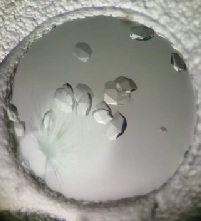
\includegraphics[width=0.3\linewidth]{../Figures/A6L.png}}
    \hfill
    \subfigure[B6,L]{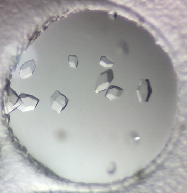
\includegraphics[width=0.3\linewidth]{../Figures/B6L.png}}
    \hfill
    \subfigure[C4,L]{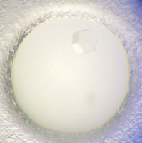
\includegraphics[width=0.3\linewidth]{../Figures/C4L.png}}
    
    \vfill % Add vertical space between rows
    
    % Second row of subfigures
    \subfigure[D4,L]{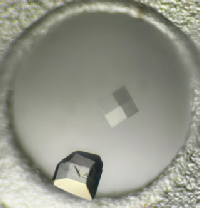
\includegraphics[width=0.3\linewidth]{../Figures/D4L.png}}
    \hfill
    \subfigure[E4,L]{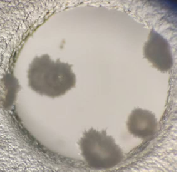
\includegraphics[width=0.3\linewidth]{../Figures/E4L.png}}
    \hfill
    \subfigure[F5,L]{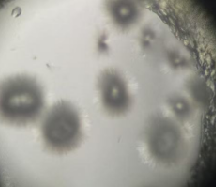
\includegraphics[width=0.3\linewidth]{../Figures/F5L.png}}
    
    \vfill % Add vertical space between rows

    % Third row of subfigures
    \subfigure[G1,L]{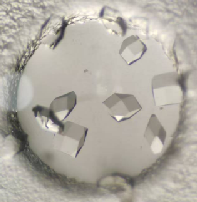
\includegraphics[width=0.3\linewidth]{../Figures/G1L.png}}
    \hfill
    \subfigure[G1,R]{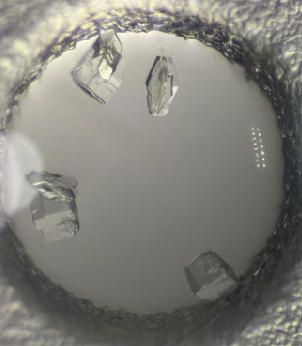
\includegraphics[width=0.3\linewidth]{../Figures/G1R.png}}
    \hfill
    \subfigure[G2,L]{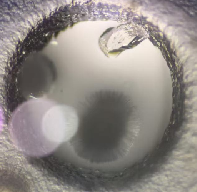
\includegraphics[width=0.3\linewidth]{../Figures/G2L.png}}
    
    \vfill % Add vertical space between rows

    % Fourth row of subfigures
    \subfigure[G2,R]{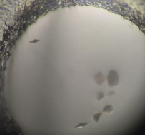
\includegraphics[width=0.3\linewidth]{../Figures/G2R.png}}
    \hfill
    \subfigure[G3,L]{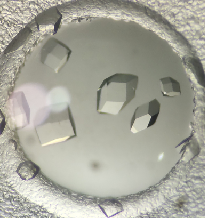
\includegraphics[width=0.3\linewidth]{../Figures/G3L.png}}
    \hfill
    \subfigure[G4,L]{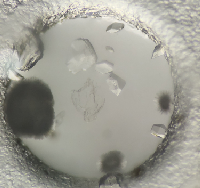
\includegraphics[width=0.3\linewidth]{../Figures/G4L.png}}
    
    \caption{Observations of Crystals}
    \label{Observations of Crystals}
\end{figure}
\section{Analysis}
\subsection{Precipitant}
Precipitants play an important role in protein Crystallization\cite{JIANG2023123187}.
In this experiment, we used inorganic salt (\ce{NaCl}) to be the precipitant.
It is commonly said that precipitation ability of salts is mainly affected by anions like \ce{Cl-} because the strongly hydrated anions may lead to protein precipitation.
Meanwhile, some articles\cite{JIANG2023123187} also point out that the cation like (\ce{Na+}) would influence the compactness and structure of lysozyme dimer and octamer, and therefore influences the crystallization.

As we had learnt from class, protein has the property of salting out.
We increased the salt concentration(Figure \ref{Configuration of Plate and Distribution of Crystals}), there must be a decrease in lysozyme solubility.

As we can see in Figure\ref{Observations of Crystals}, the crystals in D group were much larger than group A and B.
Meanwhile, the crystals in G group had a higher success rate than E and F group which were composed of mainly impurities.

I find the observations corresponds well with the theory of salting out and the solubility changing rules both in higher and lower pH.

\subsection{pH}
The pH influences the process of crystallization mainly via residues\cite{Protein_Crystallization_Wiki}.
Among the common 20 amino acids, Asp, Glu are negatively charged while Arg, Lys, His are positively charged.
The charges are produced by  carboxyl (\ce{-COOH}) and amino (\ce{-NH2}) groups which will be significantly influenced by pH.
The logic can be seen in Figure \ref{The Influence of pH}.

In our experiment, the Group E to H performed better than Group A to D averagely (larger amount and size with even shape), which means slightly higher pH is more benefit for lysozyme to crystalize.

\subsection{Protein Concentration}
In our configuration of the condition, the left cell had lower protein concentration while the right one was higher.
However, just G1 and G2 were observed with crystals on the right (higher protein concentration). Thus I suspect relatively low concentration is benefit to crystallization.
This view point was confirm by the cited article \cite{JIANG2023123187} where the scientists said the transition from non-crystal to single crystal and finally urchin-like crystal corresponds to the increase of both protein concentration and salt concentration.

\subsection{Other Aspects}
The overall success rate was relatively low, which led to fewer paralleled groups.
However, from group G we can conclude that even the experimental parameters were the same, the boundary of crystals can still be different.
This phenomenon indicates that the operational factors also contribute to the diverse results significantly.

\section{Conclusion}
In this experiment we studied the protein crystallization process with three influential factors: salt concentration, pH and protein concentration.
Relatively speaking, lower protein concentration (20 mg/mL), higher salt concentration (8\% to 10\%) and slightly higher pH (4.7) should be used for lysozyme in the pursuit of regular single crystals.




\bibliographystyle{plain}
\bibliography{references}
\end{document}